
\section{Evaluations}
\label{sec:evaluation}

We implemented a tool for TeMAPI and conducted evaluations using our tool to address the following research questions:

%\vspace*{-1.5ex}
\begin{enumerate}
%\item How effectively can existing translation tool translate API elements (Section~\ref{sec:evaluation:element})? \vspace*{-1.8ex}
\item How many API elements can be translated by existing translation tools (Section~\ref{sec:evaluation:element})? %\vspace*{-1.8ex}
%\item How effectively can our approach detect behavioral differences of single API classes (Section~\ref{sec:evaluation:single})?\vspace*{-1.8ex}
\item How many behavioral differences are effectively detected with Pex (Section~\ref{sec:evaluation:single})?%\vspace*{-1.8ex}
%\item How effectively can our approach detect behavioral differences of multiple API classes (Section~\ref{sec:evaluation:single})?\vspace*{-1.8ex}
\item How many behavioral differences are effectively detected with Randoop (Section~\ref{sec:evaluation:sequence})?%\vspace*{-1.8ex}
%\item Can the our combination strategy helps achieve better coverage (Section~\ref{sec:evaluation:coverage})?
\item How many behavioral differences are detected with and without TeMAPI's internal techniques (Section~\ref{sec:evaluation:techniques})?
\end{enumerate}%\vspace*{-1.5ex}

Table~\ref{table:subjects} shows subject tools in our evaluations. Column ``Name'' lists names of these tools. We use \emph{converter} to denote the ``VB \& C\# to Java converter'' for short. Java2CSharp, sharpen, and Net2Java are open source tools, and JLCA and converter are closed source tools. Column ``Version'' lists versions of subject tools. Column ``Provider'' lists companies of these tools. Column ``Description'' lists main functionalities of these tools. We choose these tools as subjects, since they are popular and many programmers recommend these tools in various forums.

All evaluations were conducted on a PC with Intel Qual CPU @ 2.83GHz and 2G memory running Windows XP. More details
of our evaluation results are available at \url{https://sites.google.com/site/asergrp/projects/temapi}.
\begin{table}[t]
\centering
\begin{SmallOut}
\begin {tabular} {|l|r|r|r|r|r|r|r|}
 \hline
\multicolumn{1}{|c}{\textbf{Type}}& \multicolumn{1}{|c|}{\textbf{Number}}
& \multicolumn{1}{|c|}{\textbf{Java2CSharp}} & \multicolumn{1}{|c|}{\textbf{JLCA}}& \multicolumn{1}{|c|}{\textbf{sharpen}} \\
\hline
getters of static fields      & 16,962 &   237 &  3,744 &  47 \\
\hline
setters of static fields      & 0      & 0     & 0      & 0  \\
\hline
getters of non-static fields  & 832    & 0    &   121  &  0  \\
\hline
setters of non-static fields  & 823    & 0    &   79   &  0   \\
\hline
static methods                & 1,175   & 97   &  198  &  26  \\
\hline
non-static methods            & 175,400 &3,589 &  39,536& 1,112  \\
\hline
\multicolumn{1}{|c|}{Total}   & 195,192 & 3,923 & 43,678 & 1,185\\
\hline
\end{tabular}%\vspace*{-2ex}
\Caption{Translation results of Java-to-C\# tools} \label{table:java2csharp}
\end{SmallOut}\vspace*{-6ex}
\end{table}

\subsection{Translating Synthesized Wrappers}
\label{sec:evaluation:element}
This evaluation focuses on the effectiveness of our approach to extract API mapping relations from both open source tools and closed source tools. The results are useful for subsequence steps, and also to show the effectiveness of existing translation tools. For Java-to-C\# tools, TeMAPI first synthesized wrapper methods for all classes of J2SE 6.0\footnote{\url{http://java.sun.com/javase/6/docs/api/}}. Most classes in J2SE support both generic programming and non-generic programming (\emph{e.g.}, \CodeIn{java.util.ArrayList}). During synthesis, our approach focuses on only non-generic programming as described in Section~\ref{sec:approach:wrapper}. Table~\ref{table:java2csharp} shows the translation results. Column ``Type'' lists types of synthesized methods, and Row ``Total'' denotes the sum of all methods. Column ``Number'' lists numbers of corresponding types of methods. Columns ``Java2CSharp'', ``JLCA'', and ``sharpen'' list the translation numbers of translated wrapper methods without compilation errors for each tool, respectively. Although these tools support mapping for only some APIs, these supported APIs are the most commonly used, and these tools' significant utility/popularity are reflected by their high download counts.

Our results show that JLCA is able to translate much more API elements than the other two tools. Still, even if an API element is translated, it can be translated to API elements with behavioral differences. We observe that developers of translation tools may already aware of some behavioral differences. For example, after JLCA translated synthesized code, it generated a report with many warning messages regarding behavioral differences of translated API elements. For example, a warning message was ``Method \CodeIn{java.lang.String.indexOf} was converted to \CodeIn{System.String.IndexOf}, which may throw an exception'', but the report does not describe when such an exception is thrown or how to deal with that exception. TeMAPI complements the problem, and detects that the Java method does not check whether inputs are out of ranges as the C\# method does. For example, given an empty string \CodeIn{str}, the \CodeIn{str.indexOf("", -1)} statement in Java returns 0, whereas the \CodeIn{str.IndexOf("", -1)} statement in C\# throws \CodeIn{ArgumentOutOfRangeExcpetion}.
\begin{table}[t]
\centering
\begin{SmallOut}
\begin {tabular} {|l|r|r|r|r|r|c|c|}
 \hline
\multicolumn{1}{|c}{\textbf{Type}} & \multicolumn{1}{|c}{\textbf{Number}}
& \multicolumn{1}{|c|}{\textbf{Net2Java}} & \multicolumn{1}{|c|}{\textbf{converter}}\\
\hline
getters of static fields      &  3,223 & 1    &  3     \\
\hline
setters of static fields      &  8    & 0    &  0       \\
\hline
getters of non-static fields  &   177 & 0    &  0    \\
\hline
setters of non-static fields  &   115 & 0    &  0    \\
\hline
static methods                &   996 & 0    &  6  \\
\hline
non-static methods            &190,376& 94    &  387     \\
\hline
\multicolumn{1}{|c|}{Total}   &194,835& 99     &  396 \\
\hline
\end{tabular}%\vspace*{-2ex}
\Caption{Translation results of C\#-to-Java tools} \label{table:csharp2java}
\end{SmallOut}\vspace*{-6ex}
\end{table}


For C\#-to-Java translation tools, TeMAPI first synthesized wrapper methods for all the classes of .NET framework client profile\footnote{\url{http://msdn.microsoft.com/en-us/library/ff462634.aspx}}. As described in Section~\ref{sec:approach:single}, besides generic methods, TeMAPI also ignored \CodeIn{unsafe} methods, \CodeIn{delegate} methods, and methods whose parameters are marked with \CodeIn{out} or \CodeIn{ref}. TeMAPI synthesized almost the same size of wrapper methods as it synthesized for J2SE. Table~\ref{table:csharp2java} shows the translation results. We find that both tools translate only a small number of API elements. One primary reason could be that C\# provides many features such as partial classes, reference parameters, output parameters, and named arguments, that are not provided by Java\footnote{\url{http://en.wikipedia.org/wiki/Comparison_of_Java_and_C_Sharp}}. We suspect that a C\#-to-Java translation tool needs to deal with these issues, so many mapping relations of API elements are not addressed yet.

Tables~\ref{table:java2csharp} and~\ref{table:csharp2java} show that the Java-to-C\# tools are able to translate much more API elements compared to the C\#-to-Java tools. To give more insights, we next present more details at the package level regarding the translation results of Java-to-C\# tools in Table~\ref{table:package}. Column ``Name'' lists names of Java packages. To save space, we omit 12 packages that are not translated by all the three tools (\emph{e.g.}, the \CodeIn{javax.rmi} package). Table~\ref{table:package} shows that all the three translation tools can translate the \CodeIn{java.io}, \CodeIn{java.lang}, \CodeIn{java.util}, and \CodeIn{java.net} packages. These four packages seem to be quite important for most Java programs. Almost for all these packages, JLCA translates more API elements than the other two tools. JLCA can also handle GUI-related packages such as the \CodeIn{java.awt} package and the \CodeIn{javax.swing} package, and can translate some Java programs with GUI interfaces whereas the other two tools cannot translate such programs.

\begin{table}[t]
\centering
\begin{SmallOut}
\begin {tabular} {|l|r|r|r|r|r|r|r|}
 \hline
\multicolumn{1}{|c}{\textbf{Name}}
& \multicolumn{1}{|c|}{\textbf{Java2CSharp}} & \multicolumn{1}{|c|}{\textbf{JLCA}}& \multicolumn{1}{|c|}{\textbf{sharpen}} \\
\hline
java.awt  &   0     &    8,637  &    0   \\
\hline
java.bean &   20    &    14     &    0    \\
\hline
java.io   &   592   &   1,642   &   43   \\
\hline
java.lang &   1,494  &   2,377   &   791  \\
\hline
java.math &    101   &    232    &   0    \\
\hline
java.net  &    52    &   482     &   10    \\
\hline
java.nio  &    30    &    0      &   0    \\
\hline
java.rmi  &    0     &    707   &    0   \\
\hline
java.security &  50  &    702    &  0    \\
\hline
java.sql   &   20   &     183   &   0   \\
\hline
java.text  &   96   &   321   &   0  \\
\hline
java.util  & 1,372  &   1,879   &   341   \\
\hline
javax.accesibility  &   1    &   25    &   0    \\
\hline
javax.activation     &  0    &   165   &   0     \\
\hline
javax.crypto        &   0    &    263  &    0    \\
\hline
javax.management   &   2    &    0     &   0     \\
\hline
javax.naming       &   0    &   1,365   &   0      \\
\hline
javax.security     &   0     &  619     &   0    \\
\hline
javax.sound          &   0    &   56    & 0     \\
\hline
javax.swing          &   10   &  21,364 &   0   \\
\hline
javax.xml            &   34   &   580   &   0  \\
\hline
org.omg              &   0    &  1,578  &   0    \\
\hline
w3c.dom              &   0    &   14    & 0   \\
\hline
org.xml             &    49   &   473    &  0   \\
\hline
\end{tabular}%\vspace*{-3ex}
\Caption{Java-to-C\# translation results of package level} \label{table:package}
\end{SmallOut}\vspace*{-6ex}
\end{table}
%------------------------------------------------------------
\subsection{Generating and Translating Test Cases with Pex}
\label{sec:evaluation:single}


To detect behavioral differences through wrappers, TeMAPI leverages Pex to explore safe wrappers. These methods include both the translated C\# wrapper methods without compilation errors (as shown in Table~\ref{table:java2csharp}) and the synthesized C\# wrapper methods that can be translated to Java without compilation errors (as shown in Table~\ref{table:csharp2java}). During exploration, when Pex generates inputs that exercise a feasible path in the wrapper method, TeMAPI records the inputs and resulting outputs of that path. Based on these inputs and outputs, TeMAPI generates Java test cases to ensure that synthesized wrapper methods and translated wrapper methods return the same outputs given the same inputs. Since testing GUI related API elements requires human interactions, we filter out these elements (\emph{i.e.}, the \CodeIn{awt} package and the \CodeIn{swing} package). In addition, when Pex explores methods without return values, TeMAPI ignores paths that do not throw any exceptions, since it cannot generate Java related test cases. We discuss this issue in Section~\ref{sec:discuss}.

Table~\ref{table:singleinvoc} shows the results of executing generated Java test cases. Column ``Name'' lists names of translation tools. Column ``Number'' lists numbers of generated Java test cases. Columns ``E-Tests'' and ``A-Tests'' list numbers of exception-causing and assertion-failing test cases. For the two columns, sub-columns ``M'' and ``\%'' list the number and percentages of these test cases. Table~\ref{table:singleinvoc} shows that only about half of the generated Java test cases are passed. Among the five tools, sharpen includes the lowest number of ``E-Tests'' and ``A-Tests''. It seems that programmers of sharpen put great efforts to fix behavioral differences. The percentage of JLCA is also relatively low. The results are comparable, since JLCA translates much more API elements than the other tools. In total, about 50\% of test cases are failed. These results show the effectiveness of TeMAPI, since these test cases represent behavioral differences.


For Java2CSharp, JLCA, and sharpen, we further present their testing results at the package level in Table~\ref{table:packagetest}. Column ``Name'' lists names of J2SE packages. For columns ``Java2CSharp'', ``JLCA'', and ``sharpen'', sub-column ``R'' lists numbers of generated Java test cases, and sub-column ``\%'' lists percentages of failing test cases (including exception-causing and assertion-failing). Table~\ref{table:packagetest} shows that for the \CodeIn{java.sql} and \CodeIn{java.util} packages, all tools suffer from relatively high percentages of failing test cases, and for the \CodeIn{java.lang} and \CodeIn{java.math} packages, all tools include relatively low percentages of failing test cases. This result may reflect that some packages between Java and C\# are more similar than the others, so they can be more easily translated. We also find that for the \CodeIn{java.text}, \CodeIn{javax.xml}, and \CodeIn{org.xml} packages, JLCA includes the lowest percentage of failing test cases among the five tools. The result indicates that a translation tool can achieve better translation results if its developers carefully prepare API mapping relations.


Tables~\ref{table:singleinvoc} and~\ref{table:packagetest} show that a high percentage of generated Java test cases are failed. To better understand behavioral differences between mapped API elements, we inspected 3,759 failing Java test cases. For Net2Java and converter, we inspect all failing test cases, whereas for Java2CSharp, JLCA, and sharpen, we inspect test cases generated for the \CodeIn{java.lang} package, due to a large number of failing test cases. Each failing test case reflects one unique behavioral difference, and Figure~\ref{fig:pex-percent} shows the distribution of found unique behavior differences. We next present our findings ranked by percentages of failing test cases.
\begin{table}[t]
\centering
\begin{SmallOut}
\begin {tabular} {|c|r|r|r|r|r|c|c|}
 \hline
\multirow{2}*[-2pt]{\textbf{Name}}
& \multirow{2}*[-2pt]{\textbf{Number}} & \multicolumn{2}{|c|}{\textbf{E-Tests}}& \multicolumn{2}{|c|}{\textbf{A-Tests}} \\\cline{3-6}  &  & \textbf{M}& \textbf{\%} &  \textbf{M}& \textbf{\%}\\
\hline
Java2CSharp  &   15,458 & 5,248 & 34.0\% & 3,261 & 21.1\% \\
\hline
JLCA         &   33,034 & 8,901 & 26.9\% & 6,944 & 21.0\% \\
\hline
sharpen      &  2,730 & 662  & 24.2\% & 451  & 16.5\%\\
\hline
net2java     &   352 & 40   & 11.4\%  & 261   & 74.1\%\\
\hline
converter    &  762 & 302  & 39.6\% & 182   & 23.9\%\\
\hline
Total        &  52,336  &  15,153 & 29.0\% &11,099 & 21.2\%  \\
\hline
\end{tabular}%\vspace*{-2ex}
\Caption{Results of generating C\# test cases for Java code} \label{table:singleinvoc}
\end{SmallOut}\vspace*{-6ex}
\end{table}

\textbf{Finding 1:} 36.8\% test cases show the behavioral differences caused by \CodeIn{null} inputs.

We find that many Java API methods and their translated C\# API methods have behavioral differences when \CodeIn{null} values are passed as inputs. In some cases, a Java API method can accept \CodeIn{null} values, but its translated C\# API method throws exceptions. One such example is shown in Section~\ref{sec:example} (\emph{i.e.}, the \CodeIn{skip(long)} method). In other cases, a Java API method throws exceptions given a \CodeIn{null} input, but its translated C\# API method can accept \CodeIn{null} values. For example, JLCA translates the \CodeIn{java.lang.Integer. parseInt(String,int)} method in Java to the \CodeIn{System.Convert.ToInt32(string, int)} in C\#. If the inputs of the Java method are \CodeIn{null} and $10$, it throws \CodeIn{NumberFormat- Exception}, but given the same inputs, the C\# method returns 0. We notice that translation tools can fix some differences caused by \CodeIn{null} inputs. For example, to fix the behavioral difference of \CodeIn{null} inputs for the \CodeIn{valueOf(Object)} method as shown in Section~\ref{sec:approach:single}, sharpen translates the method to its own method, and fixes the difference.

\Comment{We also find that given the same inputs, a method may produce null outputs, whereas its mapped method will not. For example, converter maps the \CodeIn{Sys- tem.Collections.Queue.ToArray()} in C\# to the \CodeIn{java.util. LinkedList.toArray()} method in Java. Given an empty list, the C\# method produce a null value, whereas the Java method produce an empty array.}

\textbf{Implication 1:} Although implementers of API libraries in different languages can come to agreements on functionalities of many API methods, behaviors for \CodeIn{null} inputs are typically controversial. Some translation tools such as sharpen try to fix these differences, however, many such differences are still left to programmers as shown in our results. Therefore, programmers should be careful when inputs are \CodeIn{null}.

\begin{table}[t]
\centering
\begin{SmallOut}
\begin {tabular} {|l|r|r|r|r|r|r|r|r|r|r|}
 \hline
\multicolumn{1}{|c}{\multirow{2}*[-2pt]{\textbf{Name}}}
& \multicolumn{2}{|c|}{\textbf{Java2CSharp}} & \multicolumn{2}{|c|}{\textbf{JLCA}}& \multicolumn{2}{|c|}{\textbf{sharpen}} \\\cline{2-7} &  \textbf{R}&  \textbf{\%} &   \textbf{R}& \textbf{\%} & \textbf{R}&   \textbf{\%}\\
\hline
java.bean &  \hfill 17     &    82.4\%  &  18        &  33.3\%   &  0      & n/a \\
\hline
java.io   &  \hfill 4,155   &  67.8\%  &  6,981       &  58.0\%   &   33    & 39.4\%\\
\hline
java.lang &  \hfill 3,480   &   37.5\%  &  4,431      &  26.1\%   &   1,753 & 29.3\%\\
\hline
java.math &  \hfill 561    &   4.3\%  &   1,629     &   1.5\%   &  0      & n/a\\
\hline
java.net  &   438     &   25.1\% &   3,941     &   47.8\%  & 9       & 44.4\%  \\
\hline
java.nio  &  \hfill 27     &  48.1\% &    0        &   n/a     &  0     &  n/a \\
\hline
java.rmi  &  \hfill 0   &   n/a   &   884     &   32.6\%  &  0     & n/a\\
\hline
java.security &  \hfill 45  &   55.6\%  &  828    &  35.6\%   &  0    & n/a \\
\hline
java.sql   &  \hfill 260&   88.1\%  & 1,465    &  91.0\%   &   0     & n/a\\
\hline
java.text  &  \hfill 566   &   61.5\%  & 374      &  18.2\%   & 0      & n/a\\
\hline
java.util  &  \hfill 5,519  &   60.8\%  & 6,177     & 70.2\%  & 935      & 62.4\%\\
\hline
javax.accessibility  &  \hfill 1    &   0.0\%   & 25         & 16.0\%    & 0          & n/a \\
\hline
javax.activation  &  0     &    n/a    & 694      & 53.9\% & 0           & n/a  \\
\hline
javax.crypto      &  0     &     n/a    & 298     & 24.2\% &  0        & n/a\\
\hline
javax.management  &  2     &    0.0\%  & 0        & n/a    &  0          & n/a  \\
\hline
naming      &  0     &    n/a     & 1,569    & 40.6\%  &  0         & n/a  \\
\hline
javax.sec.  &  0     &   n/a     & 683     & 29.4\%  &  0        & n/a\\
\hline
sound       &  0     &   n/a     & 66       & 36.4\%  &   0        &n/a  \\
\hline
javax.xml   &  110   &    71.8\%  &  628    & 45.9\%  &   0         & n/a\\
\hline
org.omg     &  0     &   n/a     & 1,842    & 36.3\%  & 0           & n/a  \\
\hline
w3c.dom     &  0     &   n/a     & 18      & 33.3\%  &  0         & n/a  \\
\hline
org.xml     &   277  &   70.0\%  & 483     & 27.3\%  & 0         & n/a\\
\hline
\end{tabular}%\vspace*{-3ex}
\Caption{Results of Table~\ref{table:singleinvoc} at package level (three tools)} \label{table:packagetest}
\end{SmallOut}\vspace*{-6ex}
\end{table}

\textbf{Finding 2:} 22.3\% test cases show the behavioral differences caused by stored \CodeIn{string} values.

We find that \CodeIn{string} values stored in fields between Java classes and their mapped C\# classes are typically different. This difference ranks as the second, since each Java class has a \CodeIn{toString()} method and each C\# class also has a \CodeIn{ToString()} method. Many translation tools map the two API methods, but the return values of the two methods are quite different in many cases. In addition, many API classes declare methods like \CodeIn{getName} or \CodeIn{getMessage}. These methods also return \CodeIn{string} values that can be quite different. In particular, we find that the \CodeIn{Message} fields of exceptions in C\# often return informative messages. One such message is ``Index was outside the bounds of the array'' provided by the \CodeIn{System.IndexOutOfRangeException.Message} field in C\#. On the other hand, exceptions in Java often provide only \CodeIn{null} messages. Overall, we find that none of the five tools fixes this difference.

\textbf{Implication 2:} Mapped \CodeIn{String} fields in different languages typically store different values, but existing translation tools do not fix those differences. Programmers should not rely on these values, since they are typically different across languages.
\begin{figure}[t]
\centering
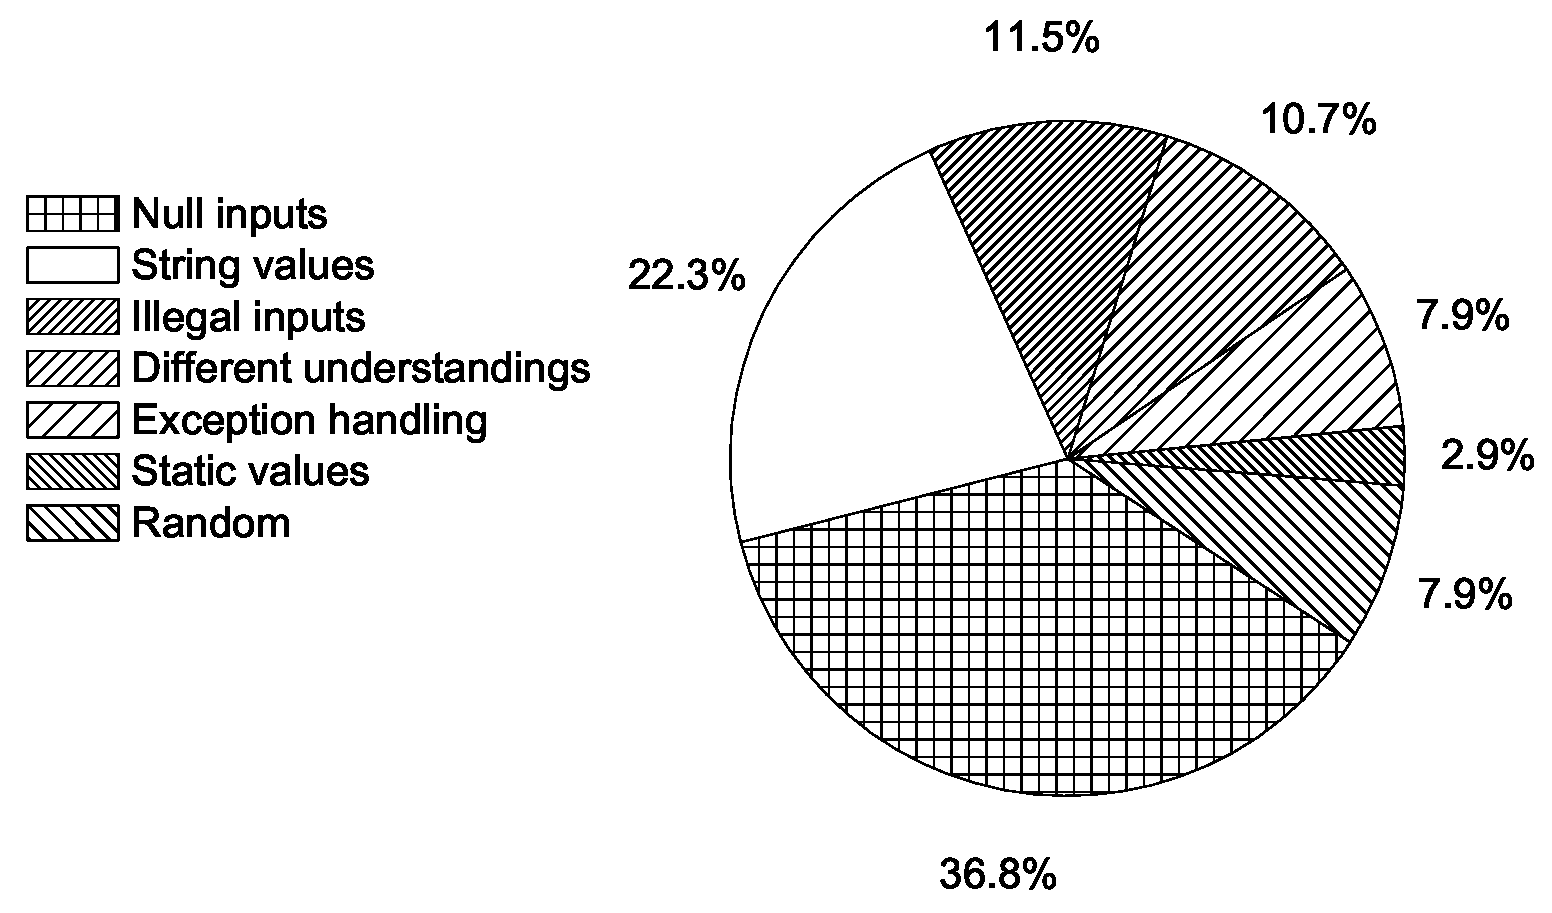
\includegraphics[scale=0.32,clip]{figure/pex-percent.eps}\vspace*{-2ex}
 \caption{Distribution of found unique behavioral differences with Pex}\vspace*{-5ex}
 \label{fig:pex-percent}
\end{figure}

\textbf{Finding 3:} 11.5\% test cases show the behavioral differences caused by different input domains.

We find that API methods in Java and API methods in C\# can have different input domains, and some legal inputs in one language can become illegal after translation. For example, the \CodeIn{java.lang.Double.shortValue()} method in Java accepts values that are larger than 32,767. JLCA translates the Java method to the \CodeIn{Convert.ToInt16 (double)} method in C\#. The C\# method throws \CodeIn{OverflowException} when values are larger than 32,767 since it checks whether inputs are too large.
As another example, the \CodeIn{java.lang.Boolean.parseBoolean(String)} method in Java does not check for illegal inputs, and returns \CodeIn{false} given an illegal input such as ``\CodeIn{test}''. Java2CSharp translates it to the \CodeIn{System.Boolean.Parse(String)} method in C\#. The C\# method throws \CodeIn{FormatException} given the same input since it checks for illegal inputs.

\textbf{Implication 3:} Mapped API methods across languages may have different input domains, and a legal input can become illegal after translation. As pointed by Cook and Dage~\cite{cook1999highly}, API translation within a single programming language also has similar problems, and a updated API method can have different input ranges with an original one. Adopting their approach may help deal with different input domains across languages.

\textbf{Finding 4:} 10.7\% test cases show the behavioral differences caused by different understandings.

We find that implementers of API libraries may have different understandings for mapped API methods in different languages. Two such examples are shown in Section~\ref{sec:approach:single} (\emph{i.e.}, the \CodeIn{capacity()} method and the \CodeIn{length()} method). In some cases, such differences reflect different natures between languages. For example, we find that Java considers ``\CodeIn{\textbackslash}'' as existing directories, but  C\# considers it not. In some other cases, we find that such differences can indicate defects in translation tools. For example, Java2CSharp translates the \CodeIn{java.lang.Integer.toHexString(int)} method in Java to the \CodeIn{ILOG.J2CsMapping.Util.IlNumber.ToString(int, 16)} method in C\#.
Given an integer -2147483648, the Java method returns ``80000000'', but the C\# method returns ``\textbackslash080000000''. As another example, Java2CSharp translates the \CodeIn{Character.isJavaIdentifierPart(char)} method in Java to the \CodeIn{ILOG.J2CsMap- ping.Util.Character.IsCSharpIdentifierPart(char)} method in C\#. Given an input ``\CodeIn{\textbackslash0}'', the Java method returns \CodeIn{true}, but the C\# method returns \CodeIn{false}. These two behavioral differences were confirmed as defects by developers of Java2CSharp after we reported the detected defects.

\textbf{Implication 4:} Implementers can have different understanding on functionalities of specific methods. Some such differences reflect different natures of different languages, and some other differences indicate  defects in translation tools. Programmers should test their translated code carefully since this type of differences is difficult to figure out.

\textbf{Finding 5:} 7.9\% test cases show the behavioral differences caused by exception handling.

We find that two mapped API methods can throw exceptions that are not mapped. For example, the \CodeIn{java.lang.StringBuffer.insert(int,char)} method in Java throws \CodeIn{ArrayIndexOutofBoundsException} when indexes are out of bounds, and Java2CSharp translates the method to the \CodeIn{System.Text.StringBuilder.Insert (int,char)} method in C\# that throws \CodeIn{ArgumentOutOfRangeException} when indexes are out of bounds. As Java2CSharp maps \CodeIn{ArrayIndexOutofBoundsException} in Java to \CodeIn{IndexOutOfRangeException} in C\#, the mapped C\# method fails to catch exceptions when indexes are out of bounds.

\textbf{Implication 5:} Implementers of API libraries may design quite different exception handling mechanisms. This type of differences is quite challenging to fix for translation tools. Even if two methods are of the same functionality, programmers should notice that these methods may produce exceptions that are not mapped.

\textbf{Finding 6:} 2.9\% test cases show the behavioral differences caused by static values.

We find that mapped static fields may have different values. For example, the \CodeIn{java. lang.reflect.Modifier} class in Java has many static fields to represent modifiers (\emph{e.g.}, \CodeIn{FINAL}, \CodeIn{PRIVATE}, and \CodeIn{PROTECTED}). Java2CSharp translates these fields to the fields of the \CodeIn{ILOG.J2CsMapping.Reflect} class in C\#. Although most values of the mapped fields are the same, we find that fields such as \CodeIn{VOLATILE} and \CodeIn{TRANSIENT} are of different values. In addition, we find that different values sometimes reveal different ranges of data types. For example, the \CodeIn{java.lang.Double.MAX\_VALUE} field in Java is 1.7976931348623157E+308, but the \CodeIn{System.Double.MaxValue} field in C\# is 1.79769313486232E+308.  Although the difference is not quite large, it can cause serious defects if a program needs highly accurate calculation results.

\textbf{Implication 6:} Implementers of API libraries may store different values in static fields. Even if two static fields have the same names, programmers should be aware of that these fields can have different values. The results also reveal that data types between Java and C\# can have different bounds. Programmers should be aware of this situation if they need highly accurate results.

The remaining 7.9\% failing test cases are related to the API methods that can return random values or values that depend on time. For example, the \CodeIn{java.util.Random. nextInt()} method returns random values, and the \CodeIn{java.util.Date.getTime()} method returns the number of milliseconds since Jan. 1st, 1970, 00:00:00 GMT. As another example, each Java class has a \CodeIn{hashCode()} method, and each C\# class has also a \CodeIn{GetHashCode()} method. Both the methods return a hash code for the current object, so translation tools such as JLCA map the two methods. Since a hash code is randomly generated, the two methods typically return different values. For these methods, TeMAPI can detect behavioral differences of their inputs. For example, converter translates the \CodeIn{System.Random.Next(int)} method in C\# to the \CodeIn{java.util. Random.nextInt(int)} method in Java. Given an integer value 0, the C\# method returns 0, but the Java method throws \CodeIn{IllegalArgumentException} with a message: ``n must be positive''. However, since these methods return values randomly, we cannot conclude that they have behavioral differences even if their outputs are different. We discuss this issue further in Section~\ref{sec:discuss}.

%--------------------------------------------------------------
\subsection{Generating and Translating Test Cases with Randoop}
\label{sec:evaluation:sequence}
\begin{table}[t]
\centering
\begin{SmallOut}
\begin {tabular} {|c|r|r|r|r|r|c|c|}
 \hline
\multirow{2}*[-2pt]{\textbf{Name}}& \multirow{2}*[-2pt]{\textbf{Method}} & \multicolumn{1}{c|}{\multirow{2}*[-2pt]{\textbf{Java}}}
& \multicolumn{1}{c|}{\multirow{2}*[-2pt]{\textbf{C\#}}} & \multicolumn{2}{|c|}{\textbf{A-Tests}} \\\cline{5-6} & &  & & \textbf{M}& \textbf{\%} \\
\hline
Java2CSharp  &  1,996 & 15,385&  2,971 & 2,151 & 72.4\%\\
\hline
JLCA         &  7,060 & 16,630& 1,067 & 295  & 27.6\%  \\
\hline
sharpen      &  586  & 13,532& 936  & 456  & 48.7\% \\
\hline
Total        &  9,642 & 45,547& 4,974  &  2,902 & 58.3\% \\
\hline
\end{tabular}%\vspace*{-2ex}
\Caption{Results of generating Java test cases for C\# code} \vspace*{-6ex}
\label{table:invocsequence}
\end{SmallOut}
\end{table}
To test behavioral differences involving invocation sequences, TeMAPI leverages Randoop to generate test cases, given the list of translatable API methods. In this evaluation, we focus on the Java-to-C\# tools only, since the C\#-to-Java tools translate only few API elements as shown in Table~\ref{table:java2csharp}. For each Java-to-C\# tool, TeMAPI first extracted the list of translatable API methods using the technique as described in Section~\ref{sec:approach:sequence}. When generating test cases, TeMAPI extends Randoop, so that each generated test case uses only translatable API methods. Randomly generated invocation sequences may not reflect API usages in true practice, and we discuss this issue in Section~\ref{sec:discuss}. Among generated test cases, we translate only passing test cases from Java to C\#.

Table~\ref{table:invocsequence} shows the results. Column ``Method'' lists sizes of translatable API methods for the three tools. Column ``Java'' lists the numbers of passing test cases in Java. Column ``C\#'' lists the numbers of translated test cases in C\#. We notice that many Java test cases are not successfully translated to C\# for two factors that are not general or not related with API migration: (1) to prepare inputs of translatable API methods, Randoop introduces API methods that are not translatable; \Comment{(2) some code structures are too complicated to translate, and we further discuss this issue in Section~\ref{sec:discuss}; }(2) the numbers of compilation errors can be magnified since Randoop produces many redundancies (Section~\ref{sec:evaluation:techniques} shows an example of produced redundancies). Our findings are as follows:

\textbf{Finding 7:} Many translated test cases have compilation errors, since Java API classes and their mapped C\# classes have different inheritance hierarchies.

We find that Java API classes can have different inheritance hierarchies with their translated C\# classes, and thus introduce compilation errors. For example, many compilation errors are introduced by type cast statements, and such an example is as follows:

\begin{CodeOut}%\vspace*{-1ex}
\begin{alltt}
public void test87() throws Throwable\{
  ...
  StringBufferInputStream var4 = ...;
  InputStreamReader var10 = new InputStreamReader((InputStream)var4, var8);
\}
\end{alltt}
\end{CodeOut}%\vspace*{-2ex}

Since the preceding two Java API classes are related through inheritance, the test case gets passed. JLCA translates the Java test case to a C\# test case as follows:

\begin{CodeOut}%\vspace*{-1ex}
\begin{alltt}
public void test87() throws Throwable\{
  ...
  StringReader var4 = ...;
  StreamReader var10 = new StreamReader((Stream)var4, var8);
\}
\end{alltt}
\end{CodeOut}%\vspace*{-2ex}

Since the two translated C\# classes have no inheritance relations, the translated C\# test case has compilation errors.

\textbf{Implication 7:} It seems to be too strict to require that implementers of API libraries in different languages follow the same inheritance hierarchy, and it is also quite difficult for translation tools to fix this behavioral difference. Programmers should deal with this difference carefully.
\begin{figure}[t]
\centering
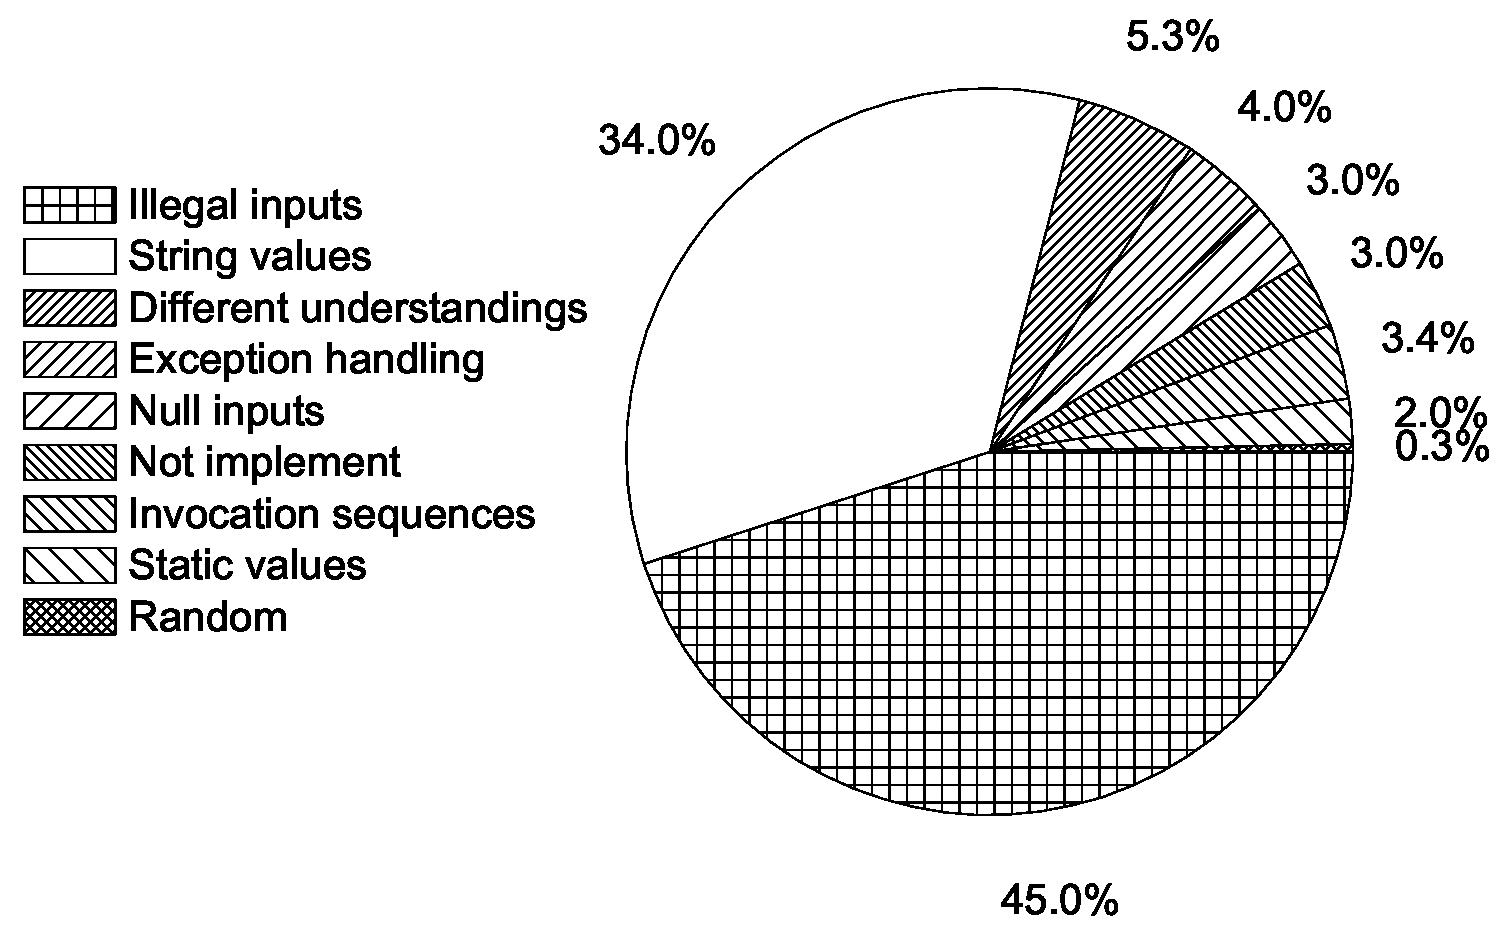
\includegraphics[scale=0.32,clip]{figure/randoop-percent.eps}\vspace*{-2ex}
 \caption{Distribution of found behavioral differences with Randoop}\vspace*{-4ex}
 \label{fig:randoop-percent}
\end{figure}

%We do not list numbers of test cases end with errors since C\# does not separate errors from failures as Java does. Sub-column ``M'' lists numbers of test cases, and sub-column ``\%'' lists percentages from failed test cases to total test cases.

Column ``A-Tests'' of Table~\ref{table:invocsequence} lists numbers and percentages of failing C\# test cases. We find that JLCA achieves the lowest percentages among the five tools. For each tool, we further investigated its first 100 failing test cases. Figure~\ref{fig:randoop-percent} shows the distribution of found behavioral differences with Randoop. We find that 93.6\% failing test cases are due to the same factors described in Section~\ref{sec:evaluation:single}: 45.0\% for ranges of parameters, 34.0\% for \CodeIn{string} values, 5.3\% for different understanding, 4.0\% for exception handling, 3.0\% for \CodeIn{null} inputs, 2.0\% for values of static fields, and 0.3\% for random values. When generating test cases, Pex explores feasible paths, whereas Randoop uses a feed-back random strategy. As a result, the distribution of Figure~\ref{fig:pex-percent} is different from the distribution of Figure~\ref{fig:randoop-percent}. The distribution of Figure~\ref{fig:pex-percent} is more reasonable since each feasible path reflects a unique behavior, and each failing test case reflects a unique behavioral difference, whereas the distribution of Figure~\ref{fig:randoop-percent} is affected by redundancies in test cases generated by Randoop. Still, Randoop's random strategy helps find an additional behavioral difference as follows:

\textbf{Finding 8:} 3.4\% test cases fail because of invocation sequences.

We find that random invocation sequences can violate specifications of API libraries. One type of such specifications is described in our previous work~\cite{zhong09:inferring}: closed resources should not be manipulated. Java sometimes allows programmers to violate such specifications although return values can be meaningless. One such example is shown in Section~\ref{sec:example} (\emph{i.e.}, the \CodeIn{test413} test case). Besides invocation sequences that are related to specifications, we find that field accessibility also leads to failures of test cases. For example, a generated Java test case is as follows:

\begin{CodeOut}%\vspace*{-1.5ex}
\begin{alltt}
public void test423() throws Throwable\{
  ...
  DateFormatSymbols var0 = new DateFormatSymbols();
  String[] var16 = new String[]{...};
  var0.setShortMonths(var16);
\}
\end{alltt}
\end{CodeOut}%\vspace*{-2ex}

JLCA translates the Java test case to a C\# test case as follows:

\begin{CodeOut}%\vspace*{-1.5ex}
\begin{alltt}
public void test423() throws Throwable\{
  ...
  DateTimeFormatInfo var0 = System.Globalization.DateTimeFormatInfo.CurrentInfo;
  String[] var16 = new String[]{...};
  var0.AbbreviatedMonthNames = var16;
\}
\end{alltt}
\end{CodeOut}%\vspace*{-2ex}

In the preceding translated test case, the last statement throws \CodeIn{InvalidOperation- Exception} since a constant value is assigned to \CodeIn{var0}.

\textbf{Implication 8:} Legal invocation sequences can become illegal after translation. The target language may be more strict to check invocation sequences, and other factors such as field accessibility can also cause behavioral differences. In most cases, programmers should deal with the difference themselves.

The remaining 3.0\% test cases get failed since translation tools such as Java2CSharp translate API elements in Java to C\# API elements that are not implemented yet. For example, Java2CSharp translates the \CodeIn{java.io.ObjectOutputStream} class in Java to the \CodeIn{ILOG.J2CsMapping.IO.IlObjectOutputStream} class in C\# that is not yet implemented, and such translations lead to \CodeIn{NotImplementException}. The evaluation in Section~\ref{sec:evaluation:single} does not detect this difference since the specific exception is not mapped.

\subsection{Significance of TeMAPI's Internal Techniques}
\label{sec:evaluation:techniques}
\begin{table}[t]
\centering
\begin{SmallOut}
\begin {tabular} {|c|r|r|r|r|r|c|c|}
 \hline
\textbf{Class}& \textbf{Method} & \textbf{Pex} & \textbf{Randoop}
& \textbf{Combination} & \textbf{Percent} \\
\hline
ParserAdapter                  &  23 &  8   & 2    &  9 & 39.1\%\\
\hline
AttributeListImpl              &  19 &  7   & 3    & 7  & 36.8\%\\
\hline
AttributesImpl                 &  31 & 15  & 11    &  18 & 58.1\%\\
\hline
XMLReaderAdapter               &  23 & 8    & 2    &  9 & 39.1\%\\
\hline
LocatorImpl                    &  17 & 4    & 0    &  4 & 23.5\%\\
\hline
DefaultHandler                 &  26 & 4    & 0    &  4 & 15.4\%\\
\hline
HandlerBase                    &  23 & 4   & 1    &  5 & 21.7\%\\
\hline
InputSource                    &  15 & 4   & 0    &  4 & 26.7\%\\
\hline
NamespaceSupport               &  15  & 5   & 2    &  6 & 40.0\%\\
\hline
SAXException                   &  15 & 5    & 1    &  5 & 33.3\%\\
\hline
SAXParseException              &  19 & 6   & 1    &  6 & 31.6\%\\
\hline
SAXNotSupportedException       &  15 & 5   & 1    &  5 & 33.3\%\\
\hline
SAXNotRecognizedException      &  15 & 5   & 1    &  5 & 33.3\%\\
\hline
Total                          &  256& 80  & 25   &  87 & 34.0\%\\
\hline
\end{tabular}%\vspace*{-2ex}
\Caption{Results with and without TeMAPI's internal techniques} \label{table:techniques}
\end{SmallOut}\vspace*{-6ex}
\end{table}

To investigate the significance of TeMAPI's internal techniques, we use JLCA as the subject tool, and the \CodeIn{org.xml} package in Java as the subject package for detecting behavioral differences. For each class of the package, we compare the number of distinct translatable methods with behavioral differences when we use TeMAPI with and without its internal techniques, and Table~\ref{table:techniques} shows the results. Column ``Class'' shows the names of classes in Java that can be translated to C\# by JLCA. Column ``Method'' lists the numbers of translatable methods of each class. These methods include inherited ones. Columns ``Pex'', ``Randoop'', and ``Combination'' list numbers of found distinct translatable methods with behavioral differences when TeMAPI uses only Pex, only Randoop, and both Pex and Randoop, respectively. With only Pex, 483 test cases were generated, and 132 test cases failed. With only Randoop, 1200 test cases were generated in Java, and all these test cases got passed. After translation, all translated test cases in C\# had no compilation errors, and 1168 C\# test cases got failed. We inspected these failing test cases, and we found that test cases generated by Pex are more effective to reveal behavioral differences than test cases generated by Randoop, since for test cases, Pex explores feasible paths whereas Randoop generates randomly. Although more test cases were generated by Randoop fail than by Pex, these failing test cases do not reveal any new methods with behavioral differences since these failing test cases are redundant. For example, we found that 1151 test cases generated by Randoop all have the same invocation sub-sequence as follows:

\begin{CodeOut}%\vspace*{-1.5ex}
\begin{alltt}
SaxAttributesSupport var25 = new SaxAttributesSupport();
System.Int32 var26 = 1;
System.String var27 = var25.GetLocalName((int) var26);
Assert.IsTrue(var27 == null);
\end{alltt}
\end{CodeOut}%\vspace*{-1.5ex}

In this sub-sequence, JLCA translates the \CodeIn{AttributeListImpl.getName(int)} method in Java to the \CodeIn{SaxAttributesSupport.GetLocalName(int)} method in C\#. The translation makes the assertion fail since the C\# method does not return \CodeIn{null} given an empty attribute as the Java method does. Besides redundancies, each test case generated by Randoop uses many API elements, and each test case generated by Pex focuses on only one field or method within a synthesized wrapper method. As a result, it takes much more efforts to locate a method with behavioral differences from failing test cases generated by Randoop than by Pex.

From the results of Table~\ref{table:techniques}, we find that Pex alone can detect most behavior differences.

However, the combination of the two techniques helps TeMAPI detect more methods with behavioral difference. Besides the behavioral differences that involve invocation sequences, we also find that Pex can fail to explore paths that are too complicated. Randoop complements Pex to generate test cases for detecting behavioral differences of such methods since Randoop generates test cases randomly. Column ``\%'' lists percentages from ``T'' to ``M''. We find that behavioral differences of mapped API methods are quite common since about one third methods have such differences.

%---------------------------------------------------------------
%\subsection{Coverage}
%\label{sec:evaluation:coverage}
%
%
%%especially in our context where most mapping relations are between J2SE and .NET Framework. For example, we find that coverage tools such as PartCover\footnote{\url{http://partcover.blogspot.com/ }} rely on the \CodeIn{JITCompilationStarted} method\footnote{\url{http://tinyurl.com/2gy2nqk}} for notifications of called methods, and thus fail to extract coverage for many methods in .NET Framework since usually no notifications are received when these method are called.
%Test coverage is a common criterion to measure the adequacy of test cases~\cite{zhu1997software}. To investigate coverage achieved by our approach with its internal techniques on and off for Java-to-C\# tools, we conduct an evaluation on JLCA. Table~\ref{table:coverageJLCA} shows the results. Column ``Class'' shows names of the subject C\# classes. JLCA generates the eight classes, and translates some classes of the \CodeIn{org.xml} package in Java to the eight C\# classes. We choose only the \CodeIn{org.xml} package in Java as the subject since it is tricky to extract coverage for internal classes of J2SE and .NET. Column ``Pex'' lists achieved coverage if TeMAPI uses only Pex to generate test cases. Column ``Randoop'' lists  achieved coverage if TeMAPI uses only Randoop to generate test cases. As Pex explores feasible paths in a systematic manner and Randoop uses random strategy, Pex achieves better coverage than Randoop except for the \CodeIn{XmlSaxLocatorImpl} class. We find that Pex can fail to generate \CodeIn{non-null} values for some interfaces. For example, the parameter of the \CodeIn{XmlSaxLocatorImpl (XmlSaxLocator)} constructor is an interface. Pex generates only \CodeIn{null} inputs for the constructor, but Randoop casts a value to the interface. As a result, Randoop achieves better coverage on this class than Pex. Still, both Pex and Randoop do not achieve high coverage for some classes (\emph{e.g.}, the \CodeIn{XmlSAXDocumentManager} class), since covering some methods requires file interactions. As both Pex and Randoop generate filenames randomly, these methods are not covered by either tool. Column ``TeMAPI'' lists the coverage achieved by combining Pex and Randoop. We find that the combination achieves the best results for all classes.
%
%To investigate coverage achieved by our approach with its internal techniques on and off for C\# to Java tools, we conduct an evaluation on converter, and Table~\ref{table:coverageconverter} shows the results.  For similar consideration, we select four classes (\emph{i.e.}, the \CodeIn{System.Collections. ArrayList} class, the \CodeIn{System.Collections.Hashtable} class, the \CodeIn{System.Collections.Queue} class, and the \CodeIn{System.Collec- tions.Stack} class). Table~\ref{table:coverageconverter} shows coverage of their translated classes in Java. The four Java classes are decompiled by JAD\footnote{\url{http://www.varaneckas.com/jad}}. We fixed compilation errors introduced during decompiling, and changed their package names. Column ``Class'' shows the names of the four Java classes. Column ``Pex'' lists achieved coverage if leveraging only Pex. We use TeMAPI to generate Java test cases when Pex explores feasible paths. Column ``Randoop'' lists  achieved coverage if leveraging only Randoop.
%%From the perspective of the four Java classes, Pex also generates test cases randomly since it does not search their feasible paths. As a result, the achieved coverage shown in Table~\ref{table:coverageconverter} are also half to half.
%Column ``TeMAPI'' lists the coverage achieved by combining Pex and  Randoop. We also find that the combination achieves the best results.
%
%\begin{table}[t]
%\centering
%\begin{SmallOut}
%\begin {tabular} {|c|r|r|r|r|r|c|c|}
% \hline
%\textbf{Class}& \textbf{Pex} & \textbf{Randoop}
%& \textbf{TeMAPI} \\
%\hline
%ManagerNotRecognizedException  &  100\% & 100\% &  100\%\\
%\hline
%ManagerNotSupportedException   &  100\% & 100\% &  100\%  \\
%\hline
%SaxAttributesSupport           &  78\%  & 74\%  &  80\%\\
%\hline
%XmlSaxDefaultHandler           &  100\% & 94\%  &  100\%\\
%\hline
%XmlSAXDocumentManager          &  29\%  & 17\%  &  29\%\\
%\hline
%XmlSaxLocatorImpl              &  83\%  & 100\%  &  100\%\\
%\hline
%XmlSaxParserAdapter            &  100\%  & 100\%  &  100\%\\
%\hline
%XmlSourceSupport               &  100\%  & 56 \%  &  100\%\\
%\hline
%\end{tabular}\vspace*{-2ex}
%\Caption{Results of testing coverage} \label{table:coverageJLCA}
%\end{SmallOut}\vspace*{-4ex}
%\end{table}

\subsection{Summary}
\label{sec:evaluation:summary}
In summary, we find that API elements are quite large in size, and translation tools typically can translate only a small portion of API elements. Although existing translation tools already notice behavioral differences of mapped API elements, many differences are not fixed. To detect behavioral differences, our approach combines random testing with dynamic-symbolic-execution-based testing, and achieves to detect more behavioral differences than with single techniques. Our approach enables us to present the first empirical comparison on behavioral differences of API mapping relations between Java and C\#. We find that various factors (\emph{i.e.}, \CodeIn{null} inputs, \CodeIn{string} values, ranges of inputs, different understanding, exception handling, static values, type cast statements, and invocation sequences) could lead to behavioral differences of mapped API elements between different languages.

\subsection{Threats to Validity}
\label{sec:evaluation:threat}
The threats to external validity include the representativeness of the subject tools. Although we applied
our approach on five popular translation tools, our approach is evaluated only on these limited tools. This threat could be reduced by introducing more subject tools in future work. The threats to internal validity include human factors for inspecting behavioral differences from failing test cases. To reduce these threats, we inspected those test cases carefully. The threat could be further reduced by involving more parties to inspect detected differences.
%\begin{table}[t]
%\centering
%\begin{SmallOut}
%\begin {tabular} {|c|r|r|r|r|r|c|c|}
% \hline
%\textbf{Class}& \textbf{Pex} & \textbf{Randoop}
%& \textbf{TeMAPI} \\
%\hline
%HashTable                      &  23\%  & 15\%  &  26\%\\
%\hline
%LinkedList                     &  32\%  & 26\%  & 37\%\\
%\hline
%ArrayList                      &  18\%  & 25\%  &  31\%\\
%\hline
%Stack                          &  21\%   & 55\%  &  55\%\\
%\hline
%\end{tabular}\vspace*{-2ex}
%\Caption{Results of testing coverage} \label{table:coverageconverter}
%\end{SmallOut}\vspace*{-4ex}
%\end{table} 